\documentclass{article}

\usepackage{nips15submit_e,times}
\nipsfinalcopy % Uncomment for camera-ready version

% General
\usepackage[numbers]{natbib}
\usepackage{setspace}
\usepackage{geometry}
\usepackage[section]{placeins}
\usepackage[hidelinks]{hyperref}
\usepackage{graphicx}
\usepackage{color}
\usepackage{titlesec}
\usepackage[page]{appendix}
\usepackage{enumerate}

% Tables/Figures
\usepackage{lscape}
\usepackage{booktabs}
\usepackage{rotating}
\usepackage{multirow}
\usepackage{longtable}
\usepackage{caption}
\usepackage{subcaption}
\usepackage{float}

% Math
\usepackage{amsmath}
\usepackage{amssymb}
\usepackage{amsthm}
\usepackage{mathtools}
\usepackage{dsfont}

%%%%%%%%%%%%%%%%%%%%%%%%%%%%%%%%%%%%%%%%%%%%%%%%%%%%%%%%%%%%%%%%%%%%%%%%%%%%%%
% User-defined LaTeX commands
\DeclareMathOperator{\Var}{Var}
\DeclareMathOperator{\Cov}{Cov}
\DeclareMathOperator{\Corr}{Corr}
\DeclareMathOperator*{\argmax}{arg\,max}
\DeclareMathOperator*{\argmin}{arg\,min}
\DeclarePairedDelimiter{\abs}{\lvert}{\rvert}
\DeclarePairedDelimiter{\norm}{\lVert}{\rVert}
\newcommand*{\expp}[1]{\exp\left(#1\right)}
\newcommand*{\foralls}{\ \forall \ }
\newcommand*{\st}{\text{ s.t. }}
\newcommand*{\E}{\mathbb E}
\newcommand*{\R}{\mathbb R}
\newcommand*{\I}{\mathds{1}}
\newcommand*{\Prob}{\mathbb P}
\newcommand*{\convas}[1]{\xrightarrow{#1}}
\newcommand*{\conv}{\convas{}}
\newcommand*{\cond}{\;\ifnum\currentgrouptype=16 \middle\fi|\;}
\newcommand*{\defeq}{%
  \mathrel{\overset{\makebox[0pt]{\mbox{\normalfont\tiny\sffamily def}}}{=}}}
\newcommand*{\notorth}{\ensuremath{\perp\!\!\!\!\!\!\diagup\!\!\!\!\!\!\perp}}
\newcommand*{\orth}{\ensuremath{\perp\!\!\!\perp}}
\newcommand*{\evalat}{\,\big\rvert}
\newcommand*{\dif}{\,\mathrm{d}}
\newcommand*{\difto}[1]{\,\mathrm{d^#1}}
\newcommand*{\difbot}[1]{\frac{\mathrm{d}}{\mathrm{d}#1}}
\newcommand*{\partialbot}[1]{\frac{\partial}{\partial#1}}
\newcommand*{\m}[1]{\textbf{#1}}
\newcommand*{\bmath}[1]{\boldsymbol{#1}}

\newcommand*{\yestag}{\addtocounter{equation}{1}\tag{\theequation}}
\newcommand*{\notaligned}[1]{\noalign{$\displaystyle #1$}}
\newcommand*{\ttilde}{{\raise.17ex\hbox{$\scriptstyle\sim$}}}
\newcommand*{\mt}[1]{\text{\normalfont #1}}

\makeatletter
\newsavebox{\mybox}\newsavebox{\mysim}
\newcommand*{\distas}[1]{%
  \savebox{\mybox}{\hbox{\kern3pt$\scriptstyle#1$\kern3pt}}%
  \savebox{\mysim}{\hbox{$\sim$}}%
  \mathbin{\overset{#1}{\kern\z@\resizebox{\wd\mybox}{\ht\mysim}{$\sim$}}}%
}
\makeatother
\newcommand*{\dist}{\sim}
\newcommand*{\distiid}{\distas{\text{i.i.d}}}

\makeatletter
\def\moverlay{\mathpalette\mov@rlay}
\def\mov@rlay#1#2{\leavevmode\vtop{%
   \baselineskip\z@skip \lineskiplimit-\maxdimen
   \ialign{\hfil$\m@th#1##$\hfil\cr#2\crcr}}}
\newcommand*{\charfusion}[3][\mathord]{
  #1{\ifx#1\mathop\vphantom{#2}\fi\mathpalette\mov@rlay{#2\cr#3}}
  \ifx#1\mathop\expandafter\displaylimits\fi}
\makeatother
\newcommand*{\cupdot}{\charfusion[\mathbin]{\cup}{\cdot}}
\newcommand*{\bigcupdot}{\charfusion[\mathop]{\bigcup}{\cdot}}

\newtheorem{theorem}{Theorem}[section]
\newtheorem{corollary}{Corollary}[section]
\newtheorem{proposition}{Proposition}[section]
\newtheorem{lemma}{Lemma}

\theoremstyle{definition}
\newtheorem{definition}{Definition}[section]
\newtheorem{example}{Example}[section]
\newtheorem*{properties}{Properties}

\newtheoremstyle{algodesc}{}{}{}{}{\bfseries}{.}{ }{}%
\theoremstyle{algodesc}
\newtheorem{algodesc}{Algorithm}
%%%%%%%%%%%%%%%%%%%%%%%%%%%%%%%%%%%%%%%%%%%%%%%%%%%%%%%%%%%%%%%%%%%%%%%%%%%%%%

\begin{document}

\title{Annealing for Mixture Models\thanks{This work was done as a final project for Stats 608A (Fall 2015) at the University of Michigan, taught by Professor Ambuj Tewari. The code used in this paper is available at \url{https://github.com/rogerfan/stochasticEM} and has been open-sourced under the Mozilla Public License, version 2.0.}}
\author{
  Joseph Dickens \\
  University of Michigan \\
  \texttt{josephdi@umich.edu} \\
\And
  Roger Fan \\
  University of Michigan\\
  \texttt{rogerfan@umich.edu} \\
}

\maketitle


\section{Introduction} \label{sec:intro}

Mixture models are a common and powerful method for clustering and distribution estimation. Data is modeled as a ``mixture'' of multiple simple distributions, most often Gaussian, where the goal is to estimate the parameters of each distribution in the mixture. In clustering problems we receive observations without knowing to which cluster they belong, a type of unsupervised learning. In this clustering setting, the alternative goal is often to estimate to which distribution each observation ``belongs.'' Mixture membership can be modeled as a latent (unobserved) variable and the model evaluated under a likelihood framework. However, because the state space of this latent variable can be extremely large (for $n$ data points from a $k$-component mixture there are $k^n$ possible latent variable realizations), direct maximization of the likelihood is generally infeasible.

The most common method used to estimate parameters in this setting is the Expectation-Maximization (EM) algorithm \cite{dempsterlairdrubin77}. The EM algorithm is an iterative optimization method used to optimize a lower bound on the likelihood. There are, however, several issues with using the EM algorithm even in this fairly simple case. Mixture models often have multiple local optima. Since EM is a hill-climbing algorithm, it may converge to a local optimum rather than a global optima \cite{wu83}. This makes EM sensitive to the chosen starting point, and various ad-hoc methods (such as multiple start or random restart) are used in practice to attempt to mitigate this issue. EM can also be slow to converge in several scenarios, including when the mixing coefficients are unbalanced or there is significant overlap in the component distributions.

In this paper, we explore other methods that attempt to mitigate EM's issues by borrowing techniques from other optimization paradigms. Simulated annealing \cite{kirkpatrickgelattvecchi83}, a stochastic method designed to find global optima in large state-spaces, is of particular interest. There have been several previous attempts to apply annealing-inspired algorithms to mixture model estimation. Most of these methods tend to mimic EM, but replace the traditional ``E-step'' with a computationally attractive alternative. Such methods seek to explore the state space without directly hill-climbing, and possibly in a non-deterministic matter. The goal is to avoid local maxima and converge to a global maxima. The most notable algorithm is Deterministic Annealing EM (DAEM), proposed by Ueda and Nakano in 1998 \cite{uedanakano98}. As the name suggests, this algorithm replaces the stochastic nature of simulated annealing with a deterministic variant to hopefully avoid the local optima problem.

We propose a new algorithm that we call Stochastic EM (SEM) and compare it to traditional EM and DAEM. We show that SEM is competitive with existing methods, and often exhibits better convergence rates on average. When the computing budget is high enough SEM can converge to significantly higher-likelihood states than EM or DAEM. However, due to its stochastic nature, SEM is not well-suited for all situations.


\section{Previous Algorithms} \label{sec:prev_algos}


\subsection{Expectation-Maximization}

In their paper first proposing the general EM Algorithm \cite{dempsterlairdrubin77}, Dempster et. al. demonstrate its applicability to mixture model estimation, and EM has become the standard method of estimating parametric finite mixture models.

Assume that data vectors $X_1, \dots, X_n$ are i.i.d. draws from the $J$-component mixture distribution
\begin{equation*}
P(X) = \sum_{j=1}^J \pi_j P_j(X \cond \theta_j)
\end{equation*}
Where $\pi_j$ are the mixing components, $P_j$ are the individual probability distributions, each indexed by a parameter vector $\theta_j$. Note that we can reparameterize this model by introducing a latent variable $Z$ that indicates group membership. Then our data generating model becomes:\footnote{Note that $\mt{Mult}(\cdot)$ here refers to the Multinomial distribution with $n=1$ trials, otherwise known as the Categorical distribution.}
\begin{align*}
Z &\dist \mt{Mult}(\pi_1, \dots, \pi_J) \\
X \cond Z &\dist P_Z
\end{align*}
For simplicity, in this paper we will assume that the base distributions are multivariate Gaussian, so the parameters are $\theta_j = (\mu_j, \Sigma_j)$. Gaussian mixture models are by far the most commonly used in practice, but the algorithms and methods in this paper generalize to many base distributions.

To estimate this model, we can use the EM algorithm as follows:
\begin{enumerate}
\item Initialize parameters for each distribution $\mu_j^{(0)}$, $\Sigma_j^{(0)}$, and mixing components $\pi_j^{(0)}$.
\item Iterate the following steps until convergence or a computing budget is met:
  \begin{enumerate}
  \item E-step: Estimate the membership probabilities $p_{ij}^{(k+1)}$ for each observation $i$ using the current parameter estimates $\mu_j^{(k)}$, $\Sigma_j^{(k)}$ and mixing components $\pi_j^{(k)}$.
    \begin{equation} \label{eq:em_estep}
    p_{ij}^{(k+1)} = P(Z_i = j \cond X_i, \mu^{(k)}, \Sigma^{(k)}, \pi^{(k)})
      = \frac{\pi_j^{(k)} P_j(X_i \cond \mu_j^{(k)}, \Sigma_j^{(k)})}{\sum_{j'=1}^J \pi_{j'}^{(k)} P_{j'}(X_i \cond \mu_{j'}^{(k)}, \Sigma_{j'}^{(k)})}
    \end{equation}
  \item M-step: Estimate the parameters and mixing components using maximum likelihood estimation conditional on the current membership probabilities.
    \begin{equation} \label{eq:em_mstep}
    \begin{gathered}
    \pi_j^{(k+1)} = \frac{1}{n} \sum_{i=1}^n p_{ij}^{(k+1)} \qquad
    \mu_j^{(k+1)} = \frac{\sum_{i=1}^n p_{ij}^{(k+1)} X_i}{\sum_{i=1}^n p_{ij}^{(k+1)}} \\
    \Sigma_j^{(k+1)} = \frac{\sum_{i=1}^n p_{ij}^{(k+1)} (X_i - \mu_j^{(k+1)}) (X_i - \mu_j^{(k+1)})'}{\sum_{i=1}^n p_{ij}^{(k+1)}}
    \end{gathered}
    \end{equation}
  \end{enumerate}
\end{enumerate}


\subsection{Issues with EM} \label{subsc:em_issues}

Despite its power and ubiquity, the EM algorithm is known to struggle in several common scenarios. Ueda and Nakano show that when clusters have significant overlap, convergence of EM tends to be much slower than when clusters are well separated in the data space \cite{uedanakano98}. Unfortunately, interesting problems are generally those with overlap, since unsupervised learning problems are much more difficult in these settings. Additionally, Naim and Gildea show that when mixing probabilities are unbalanced, i.e. when one or more classes have small mixing coefficients, EM can be very slow to converge as well \cite{naimgildea12}.

Figure~\ref{fig:em_struggles} demonstrates the effects of these issues with some simple comparisons. When the mixing components are unbalanced or there are significantly overlapping distributions, the EM algorithm tends to get stuck in slow-convergence areas, likely near saddle points. In the easier settings, the EM algorithm moves towards its limit much more quickly. In both of these cases the EM algorithm eventually escapes and converges to the maximum, but the convergence rate is severely effected.

\begin{figure}[htb] \centering
  \begin{subfigure}[t]{.45\linewidth}
    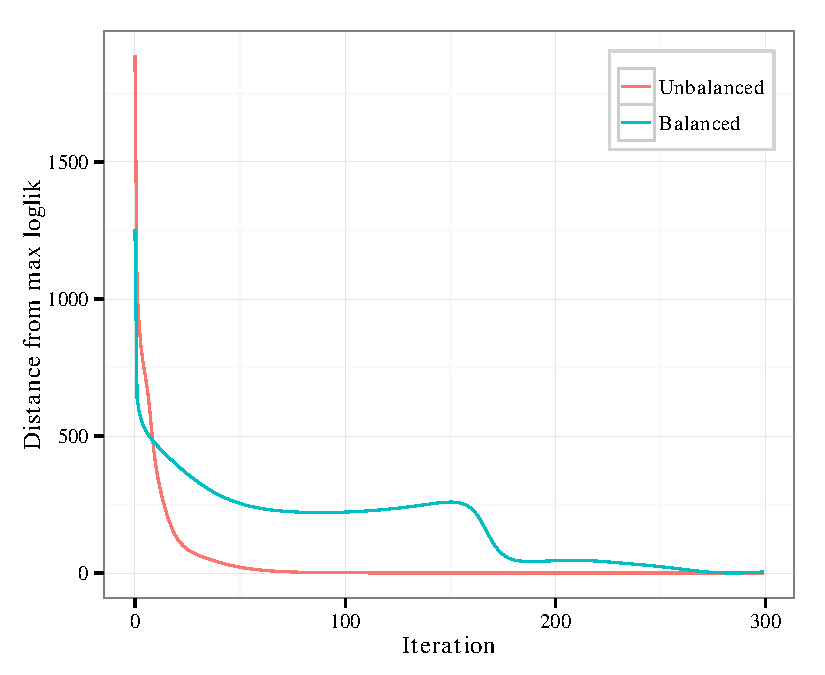
\includegraphics[width=\linewidth]{include/em_imbalance.pdf}
    \caption{Unbalanced Mixing} \label{fig:em_struggles_unbal}
  \end{subfigure}
  \begin{subfigure}[t]{.45\linewidth}
    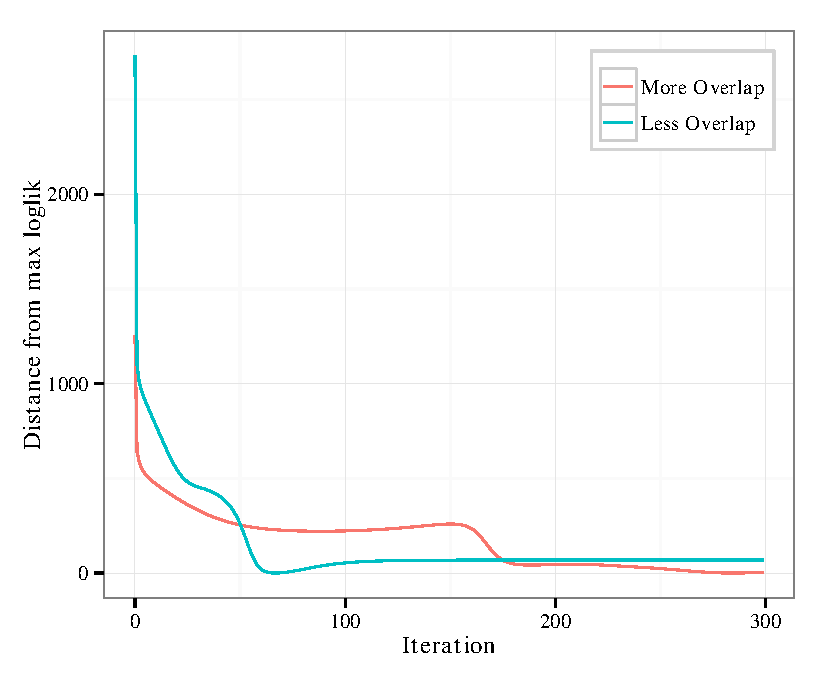
\includegraphics[width=\linewidth]{include/em_overlap.pdf}
    \caption{Overlapping Distributions} \label{fig:em_struggles_overlap}
  \end{subfigure}
  \caption{Situations where the EM algorithm has convergence issues.}
  \label{fig:em_struggles}
\end{figure}


\subsection{Deterministic Annealing}

Ueda and Nakano proposed a modification of the EM algorithm that they call Deterministic Annealing Expectation Maximization (DAEM) \cite{uedanakano98}. This algorithm is inspired by both simulated annealing and the EM algorithm, and introduces an inverse temperature parameter $\beta$ that determines how ``smoothed'' the clusters are. The DAEM algorithm is the same as EM, except replacing Equation~\ref{eq:em_estep} (the E-step) with
  \begin{equation} \label{eq:da_estep}
  p_{ij}^{(k+1)}
    = \frac{\left( \pi_j^{(k)} P_j(X_i \cond \mu_j^{(k)}, \Sigma_j^{(k)}) \right)^{\beta_k}}{\sum_{j'=1}^J \left( \pi_{j'}^{(k)} P_{j'}(X_i \cond \mu_{j'}^{(k)}, \Sigma_{j'}^{(k)}) \right)^{\beta_k}}
  \end{equation}

Note that when $\beta = 0$ the posterior membership probabilities become uniform, and when $\beta = 1$ we recover the standard EM algorithm. Generally we choose $\beta_0$ to be small, which does some smoothing between clusters, and allow $\beta_k \to 1$ as our iterations increase.

% The hope is that, by initially optimizing over the smoothed version of the likelihood, local optima and saddle points can be avoided. Unfortunately, initial progress is much slower until $\beta$ gets close to 1, but by avoiding the slow convergence areas shown in Figure~\ref{fig:em_struggles} overall convergence is likely improved.


\section{Simulated Annealing} \label{sec:simanneal}

Simulated annealing is a stochastic optimization algorithm designed to find global optima in optimization problems with large state spaces \cite{kirkpatrickgelattvecchi83}. Consider the maximization problem
\begin{equation*}
x^* = \argmax_{x \in \Omega} f(x)
\end{equation*}
The general simulated annealing algorithm proceeds as follows:
\begin{enumerate}
\item Initialize at some point $x^{(0)}$ and initial temperature $T_0$.
\item Repeat until a computing budget is met:
  \begin{enumerate}
  \item Consider some stochastically chosen candidate point $x = g(x^{(k)})$.
  \item If $f(x) > f(x^{(k)})$, accept the candidate move and set $x^{(k+1)} = x$.
  \item Otherwise, accept the candidate move with probability $e^{(f(x) - f(x^{(k)})/T_k}$.
  \item If the candidate move is not accepted, then stay at the current point $x^{(k+1)} = x^{(k)}$.
  \item Cool the temperature $T_{k+1} = \alpha T_k$ for some $0 \ll \alpha < 1$.
  \end{enumerate}
\end{enumerate}

Note that the current temperature $T_k$ determines how willing the algorithm is to accept moves that lower the objective function. For high temperatures, the algorithm accepts almost any move and uses this to explore the state space. As the temperature cools, the algorithm tends towards objective-improving moves and hopefully converges to the global optima.

In order to apply this algorithm to mixture models, we consider possible values of the latent mixture membership variable $Z$ as the state space to optimize over. Given a realization of $Z$, we can write the log-likelihood function as
\begin{equation*}
\log P(X) = \sum_{i=1}^n \sum_{j=1}^J \I(Z_i = j) \log P_j(X_i \cond \theta_j)
\end{equation*}
Plugging in the MLE estimates for $\theta_j$ conditional on $Z$, we therefore can apply simulated annealing to the objective function
\begin{equation} \label{eq:sa_obj}
f(Z) = \sum_{i=1}^n \sum_{j=1}^J \I(Z_i = j) \log P_j(X_i \cond \hat{\theta}_j)
\end{equation}

% In order to implement simulated annealing to estimate mixture models, we must find a method of selecting new candidate realizations of $Z$. The implementation that adheres most closely to the traditional simulated annealing algorithm stated above randomly selects one observation and switches its membership. In this practice we found that the number of switches required to to achieve convergence made the method uncompetitive with existing algorithms. Instead, we will again draw inspiration from the EM algorithm in order to develop a simulated annealing approach that updates the entire dataset at once.


\subsection{Stochastic EM}

We propose a new algorithm that we call Stochastic EM (SEM). This is an implementation of simulated annealing that randomly draws new realizations for the entire $Z$ vector at each iteration. The SEM algorithm roughly follows the same structure as the EM algorithm:
\begin{enumerate}
\item Initialize parameters for each distribution $\mu_j^{(0)}$, $\Sigma_j^{(0)}$, mixing components $\pi_j^{(0)}$, and choose an initial temperature $T_0$.
\item Iterate the following steps until a computing budget is met:
  \begin{enumerate}
  \item Estimate the membership probabilities $p_{ij}^{(k+1)}$ using the current parameter estimates $\mu_j^{(k)}$, $\Sigma_j^{(k)}$ and mixing components $\pi_j^{(k)}$. Note that this is the exact same calculation as Equation~\ref{eq:em_estep}, the E-step from the EM algorithm.
  \item Randomly draw candidate memberships $\tilde{Z} = (\tilde{Z}_1, \dots,\tilde{Z}_n)'$, where
    \begin{equation*}
    \tilde{Z}_i \dist \mt{Mult}\left(p_{i1}^{(k+1)}, \dots, p_{iJ}^{(k+1)}\right)
    \end{equation*}
  \item Estimate candidate parameters and mixing components using maximum likelihood estimation conditional on the memberships $\tilde{Z}$. This is analagous to the M-step in EM (\ref{eq:em_mstep}).
    \begin{equation} \label{eq:sa_mstep}
    \begin{gathered}
    \tilde{\pi}_j = \frac{1}{n} \sum_{i=1}^n \I(\tilde{Z}_i = j) \qquad
    \tilde{\mu}_j = \frac{\sum_{i=1}^n \I(\tilde{Z}_i = j) X_i}{\sum_{i=1}^n \I(\tilde{Z}_i = j)} \\
    \tilde{\Sigma}_j = \frac{\sum_{i=1}^n \I(\tilde{Z}_i = j) (X_i - \tilde{\mu}_j) (X_i - \tilde{\mu}_j)'}{\sum_{i=1}^n \I(\tilde{Z}_i = j)}
    \end{gathered}
    \end{equation}
  \item Calculate the candidate objective function
    \begin{equation*}
    f(\tilde{Z}) = \sum_{i=1}^n \sum_{j=1}^J \I(\tilde{Z}_i = j) \log P_j(X_i \cond \tilde{\mu}_j, \tilde{\Sigma}_j)
    \end{equation*}
  \item Update:
    \begin{enumerate}
    \item If $f(\tilde{Z}) > f(Z^{(k)})$ then accept the candidate memberships and update
      \begin{align*}
      Z^{(k+1)} &= \tilde{Z} & \pi^{(k+1)} &= \tilde{\pi} \\
      \mu^{(k+1)} &= \tilde{\mu} & \Sigma^{(k+1)} &= \tilde{\Sigma}
      \end{align*}
    \item Otherwise, acccept the candidate memberships with probability $e^{(f(x) - f(x^{(k)})/T_k}$.
    \item If the candidate move is not accepted, then stay at the current point $Z^{(k+1)} = Z^{(k)}$.
    \end{enumerate}
  \item Cool the temperature $T_{k+1} = \alpha T_{k}$.
  \end{enumerate}
\item Since the algorithm can accept worsening moves, return the function value and parameters associated with the best-so-far iteration $k^* = \argmin_{k} f(Z^{(k)})$.
\end{enumerate}

SEM is effectively a discrete, stochastic version of EM. Instead of using the membership probabilities, SEM only allows for discrete memberships and randomly chooses memberships at each iteration using the estimated probabilities. Due to this inaccuracy, we expect that the SEM will lose some convergence speed relative to standard EM, but hope that its discrete and stochastic nature will help it avoid local optima and saddle points.


\section{Results} \label{sec:results}


\subsection{Data Generation}

We simulate data from a 3-component Gaussian mixture model to compare these methods with. In order to provide a more challenging optimization environment, we include significant overlap and somewhat unbalanced mixing coefficients.\footnote{In particular, we set $\mu_1 = (0, 2)'$, $\mu_2 = (2, 1)'$, $\mu_3 = (2, 3)'$; $\Sigma_1 = \begin{pmatrix} 1 & 0.1 \\ 0.1 & 0.3 \end{pmatrix}$, $\Sigma_2 = \begin{pmatrix} 1 & -0.1 \\ -0.1 & 1 \end{pmatrix}$, $\Sigma_3 = \begin{pmatrix} 0.5 & -0.5 \\ -0. & 1 \end{pmatrix}$; and $\pi_1 = 0.15$, $\pi_2 = 0.70$, $\pi_3 = 0.15$.} Figure~\ref{fig:sim_data} shows an example of $n=2000$ draws from our mixture model. The majority of our analysis will be run on this data set.

\begin{figure}[t] \centering
  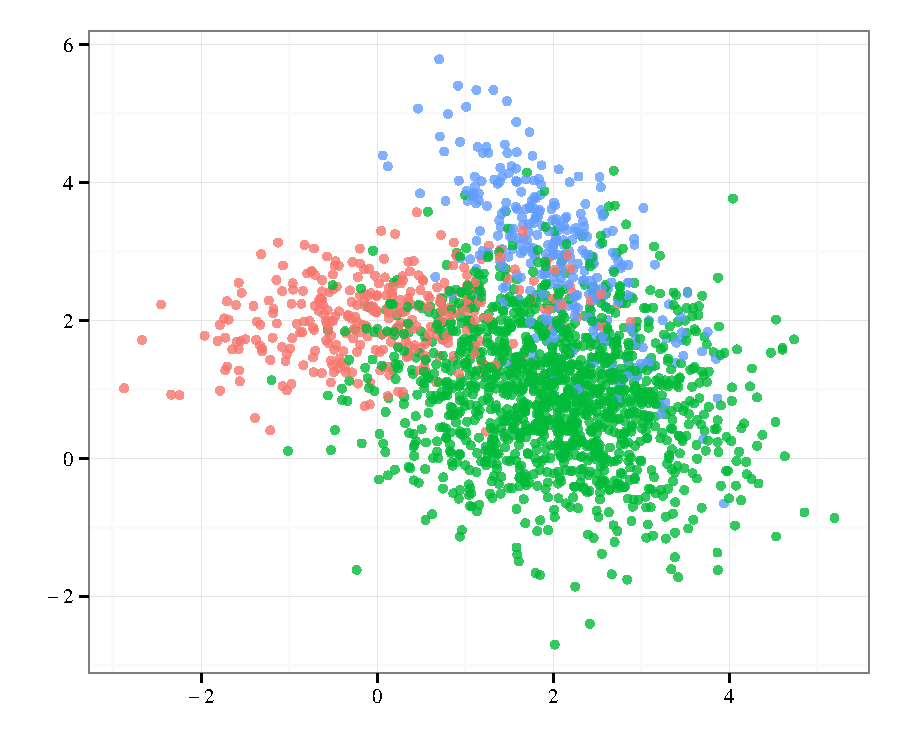
\includegraphics[width=.45\linewidth]{include/sim_data.pdf}
  \caption{2000 draws from our 3-component Gaussian mixture model.}
  \label{fig:sim_data}
\end{figure}


\subsection{Simulation results}

Figure~\ref{fig:algcomps} shows the results of EM, DAEM, and SEM runs using the same initial parameter values for each algorithm.\footnote{SEM is estimated using an initial temperature of $T_0 = 100$ and a cooling schedule of $\alpha = 0.992$.} We see that the EM algorithm exhibits the same issues described in Section~\ref{subsc:em_issues}, where the algorithm is caught in a slow-convergence area for a significant number of iterations. As expected, DAEM has slower initial convergence due to the smoothing of membership probabilities, but avoids slow-convergence areas and has better overall convergence performance.

\begin{figure}[htb] \centering
  \begin{subfigure}[t]{.45\linewidth}
    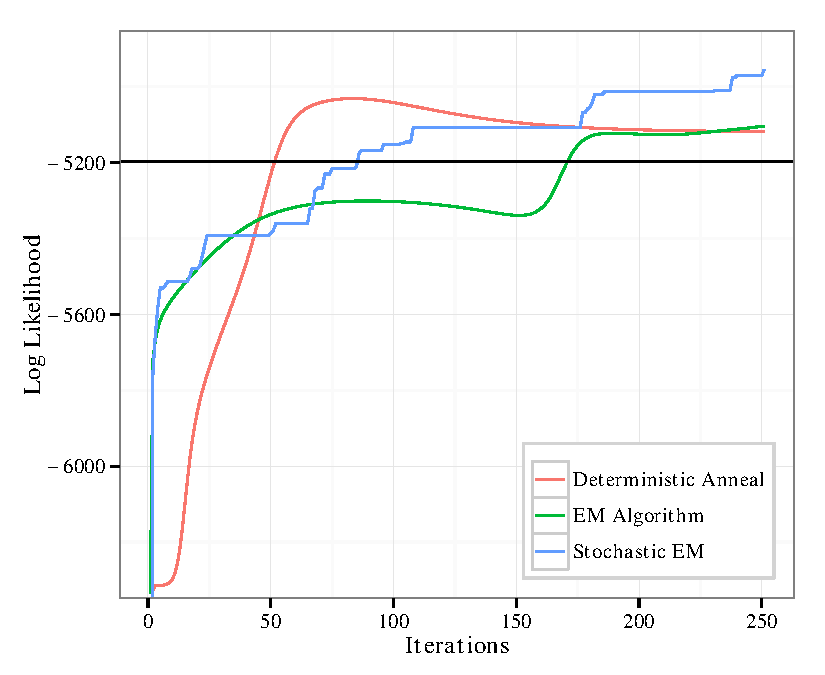
\includegraphics[width=\linewidth]{include/results_byiter.pdf}
    \caption{By Iterations} \label{fig:algcomps_byiter}
  \end{subfigure}
  \begin{subfigure}[t]{.45\linewidth}
    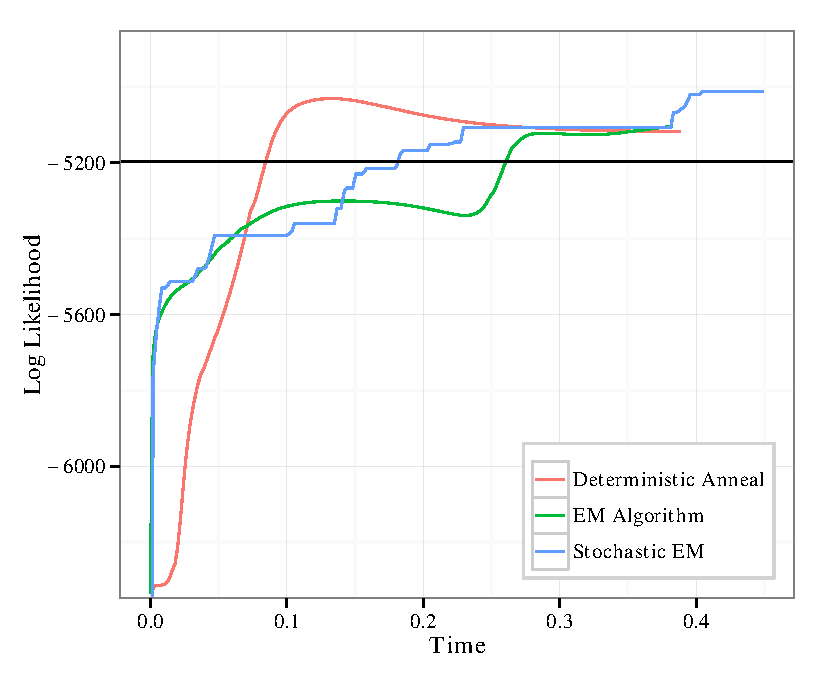
\includegraphics[width=\linewidth]{include/results_bytime.pdf}
    \caption{By Time} \label{fig:algcomps_bytime}
  \end{subfigure}
  \caption{Convergence performance of EM, DAEM, and SEM on the dataset shown in Figure~\ref{fig:sim_data}, by both iteration number and processor time.}
  \label{fig:algcomps}
\end{figure}

Stochastic EM seems to be fairly competitive with EM and DAEM, striking a middle point between the two. It attains the fast initial convergence of EM, but its stochastic nature allows it to escape the slow convergence area more quickly than regular EM. It also reaches a significantly higher final likelihood than either of the two other algorithms. Figure~\ref{fig:algcomps_bytime} shows how each of the algorithms performs against time. Stochastic EM adds some computation to each step, but is still competitive with the other two methods. All three algorithms have the same order of computational complexity per iteration.

\begin{figure}[htb] \centering
  \begin{subfigure}[t]{.45\linewidth}
    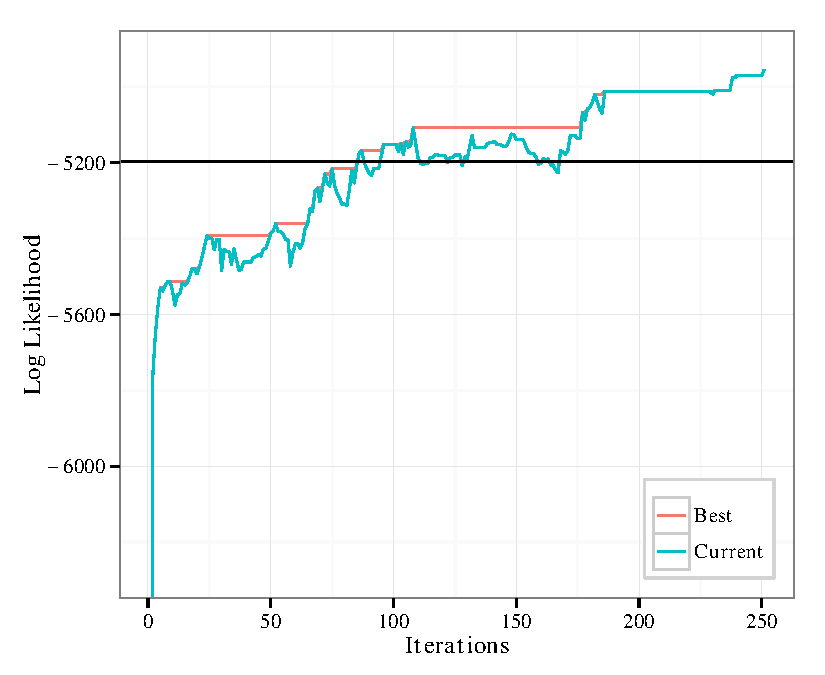
\includegraphics[width=\linewidth]{include/sa_singlerun.pdf}
    \caption{Single SEM Run} \label{fig:sa_singlerun}
  \end{subfigure}
  \begin{subfigure}[t]{.45\linewidth}
    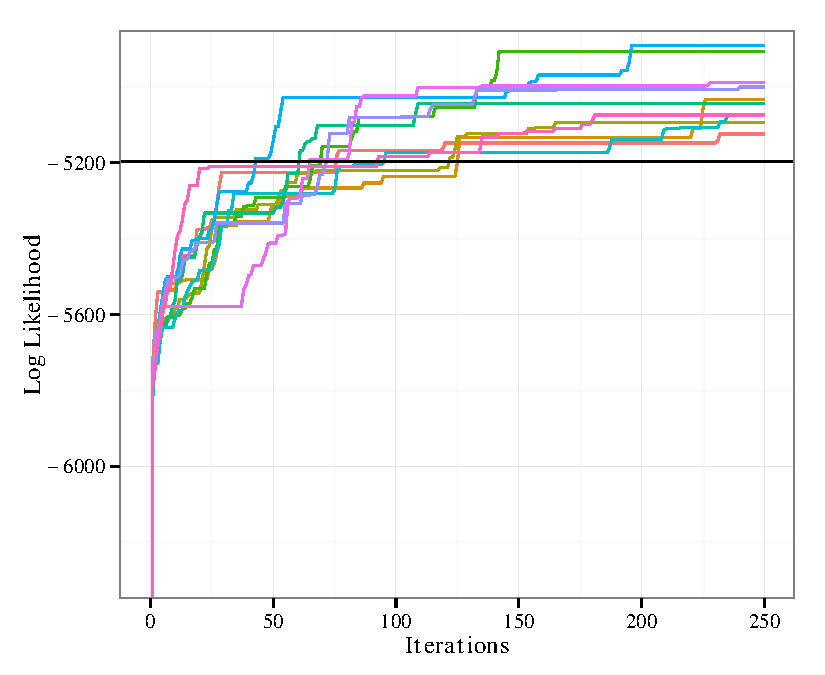
\includegraphics[width=\linewidth]{include/sa992.pdf}
    \caption{Multiple SEM Runs} \label{fig:sa_multrun}
  \end{subfigure}
  \caption{SEM run examples. (\subref{fig:sa_singlerun}) compares the best-so-far log-likelihood to the log-likelihood of the current position. (\subref{fig:sa_multrun}) shows multiple SEM runs from the same initial values.}
  \label{fig:sa}
\end{figure}

Figure~\ref{fig:sa_singlerun} shows how the likelihood of the current position (as opposed to the best-so-far) evolves in SEM. We can see that the algorithm's ability to accept objective-worsening moves allows it to further explore the state space and hopefully find better areas despite non-convexity.

We must keep in mind, however, that SEM is a stochastic algorithm. Figure~\ref{fig:sa_multrun} shows 10 example SEM runs on this data set, each using the exact same initial values. The final likelihood for even the worst-case SEM run is similar to those attained by EM and DAEM, but there is significant spread in both the convergence speed and final values. With enough computational time and slow enough cooling the algorithm should attain similar final results, but its stochastic nature means that it may not be well-suited for some applications.

\begin{figure}[hbt] \centering
  \begin{subfigure}[t]{.45\linewidth}
    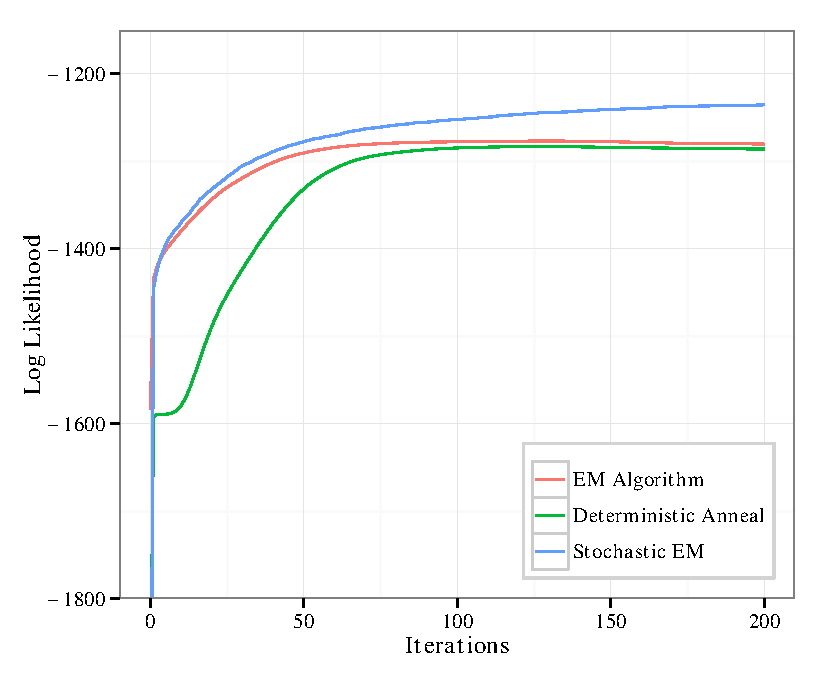
\includegraphics[width=\linewidth]{include/avg_lik_500.pdf}
    \caption{$n=500$} \label{fig:sims_n500}
  \end{subfigure}
  \begin{subfigure}[t]{.45\linewidth}
    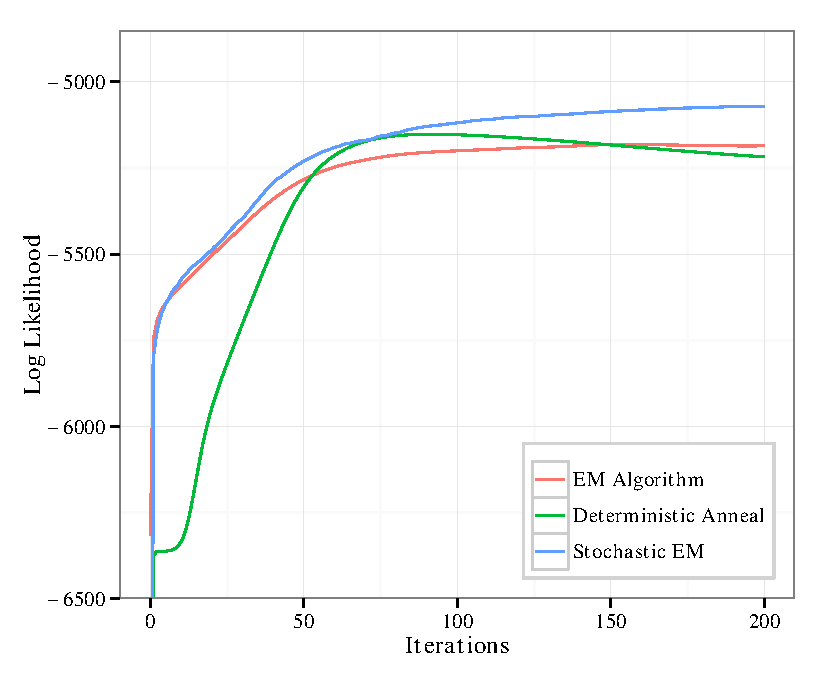
\includegraphics[width=\linewidth]{include/avg_lik_2000.pdf}
    \caption{$n=2000$} \label{fig:sims_n2000}
  \end{subfigure}
  \caption{Average log-likelihood for each algorithm over 100 simulated datasets.}
  \label{fig:sims}
\end{figure}

% \begin{table}[hb]
% \centering
% \begin{tabular}{rrrr}
%   \hline
% Method            & SEM   & EM    & DAEM \\
% \hline
% Average Distance  & 0.49  & 0.47  & 0.20 \\
%    \hline
% \end{tabular}
% \caption{Average distance between true cluster means and estimates}
% \label{tab:mu_distance}
% \end{table}

To further explore the effectiveness of SEM, we compared all three optimization methods on 100 simulated datasets for varying sample sizes. Figure~\ref{fig:sims} shows the average log-likelihoods of each method for these simulations. We can see that, on average, SEM is competitive with or outperforms both EM and DAEM. DAEM in particular seems to perform worse for smaller data sets, but has competitive performance with larger sample sizes. Once again, we see that SEM might overfit the data, since it converges to a higher final log-likelihood. We are primarily interested in whether the algorithms can recover the true mixture means.
% To check to see if each algorithm did, over 100 runs, we calculated the average distance from each estimated cluster mean to true cluster mean. The results are found in Table~\ref{tab:mu_distance}, where we see that DAEM outperforms both EM and SEM at estimating mixture means. Perhaps more importantly, SEM performs comparably to EM, making it a competitive alternative for certain applications.

\section{Conclusion} \label{sec:conclusion}

Expectation-Maximization and EM-based algorithms are some of the most common methods for estimating mixture models. Existing deterministic methods, however, struggle to optimize in some conditions. The non-convex nature of mixture model likelihoods means that local optima or saddle points can stop or significantly slow down optimization progress. In this paper, we introduce a novel algorithm for estimating mixture models that we call Stochastic EM. This algorithm applies simulated annealing principles to the EM algorithm to hopefully avoid these issues and achieve more consistent global optimization. We implement SEM for Gaussian mixture models and show that it is competitive with existing algorithms and often out-performs them on-average. There are some tradeoffs, but SEM seems to be a promising alternative algorithm for estimating mixture models.

% Statisticians rely on so-called ``workhorse'' algorithms as the basis for much of their work, and make small adjustments when these reliable algorithms do not perform as well as they expect. This paper is one such attempt to modify the EM algorithm, usually one's first choice when estimating a mixture model. Generally reliable, its convergence slows when mixtures are unbalanced or overlapping. The literature is filled with modifications that help improve convergence by slightly modifying the traditional EM by attempting to counteract EM's tendency to converge to local optima.We have made a similar contribution by introducing a stochastic EM algorithm, which uses stochasticity to remove itself from local optima and converge more quickly to a global optima. Finally, we have shown that SEM is computationally competitive with other modified EM algorithms and estimates Gaussian mixture means well in practice.


% \vfill
% \FloatBarrier \pagebreak
% \nocite{*}
\bibliographystyle{unsrt}
\bibliography{biblio}


\end{document}
